%!TEX root = ../thesis.tex
\documentclass[../thesis]{subfiles}

\begin{document}
	\section{Results}
	\label{sec:multicore:results}

	\Cref{fig:multicore:point:row:times} shows the execution times obtained for the point method with the row strategy. Preliminary tests with the column strategy showed identical results. It is clear that these strategies does not scale at all, unlike what happens with the diagonal strategy (\cref{fig:multicore:point:diagonal:times}), which reaches its maximum performance when using all the hardware supported threads.

	\begin{figure}[hp]
		\begin{center}
			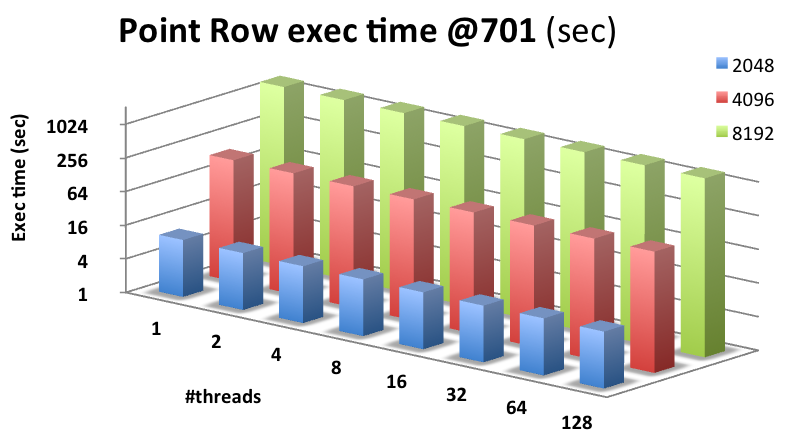
\includegraphics[width=0.9\textwidth]{assets/images/multicore/point-row.png}
		\end{center}
		\caption{Execution times for point method and row strategy}
		\label{fig:multicore:point:row:times}
	\end{figure}

	\begin{figure}[hp]
		\begin{center}
			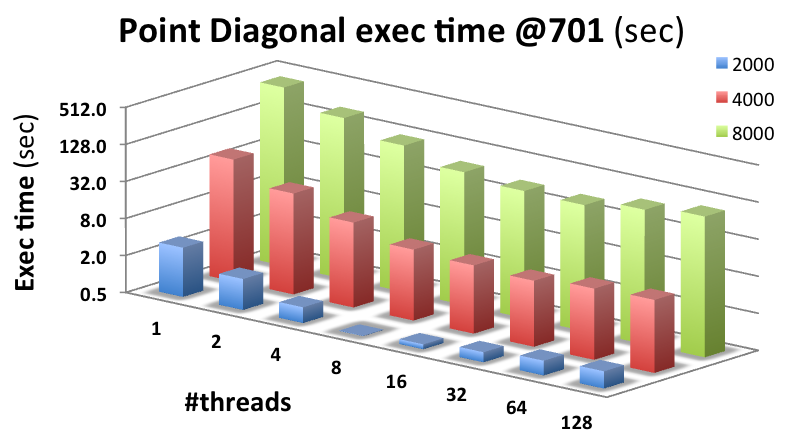
\includegraphics[width=0.9\textwidth]{assets/images/multicore/point-diagonal.png}
		\end{center}
		\caption{Execution times for point method and diagonal strategy}
		\label{fig:multicore:point:diagonal:times}
	\end{figure}

	The block method (\cref{fig:multicore:block:diagonal:times}) also scales well, with the minimum execution time being reached when using 32 threads (the 16 cores with Hyper-Threading). \Cref{fig:multicore:sensitivity} shows that the block method not only is faster than the point method, it is also less sensitive to small variations in the matrix size.

	\begin{figure}[hp]
		\begin{center}
			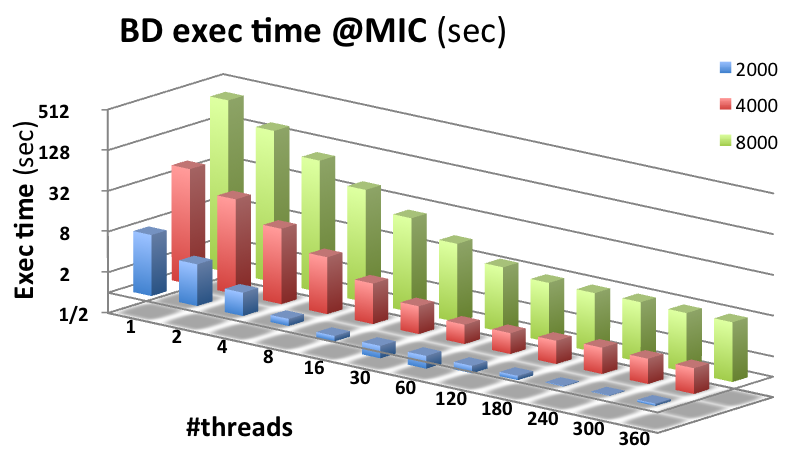
\includegraphics[width=0.9\textwidth]{assets/images/multicore/block-diagonal.png}
		\end{center}
		\caption{Execution times for block method and diagonal strategy}
		\label{fig:multicore:block:diagonal:times}
	\end{figure}

	\begin{figure}[hp]
		\begin{center}
			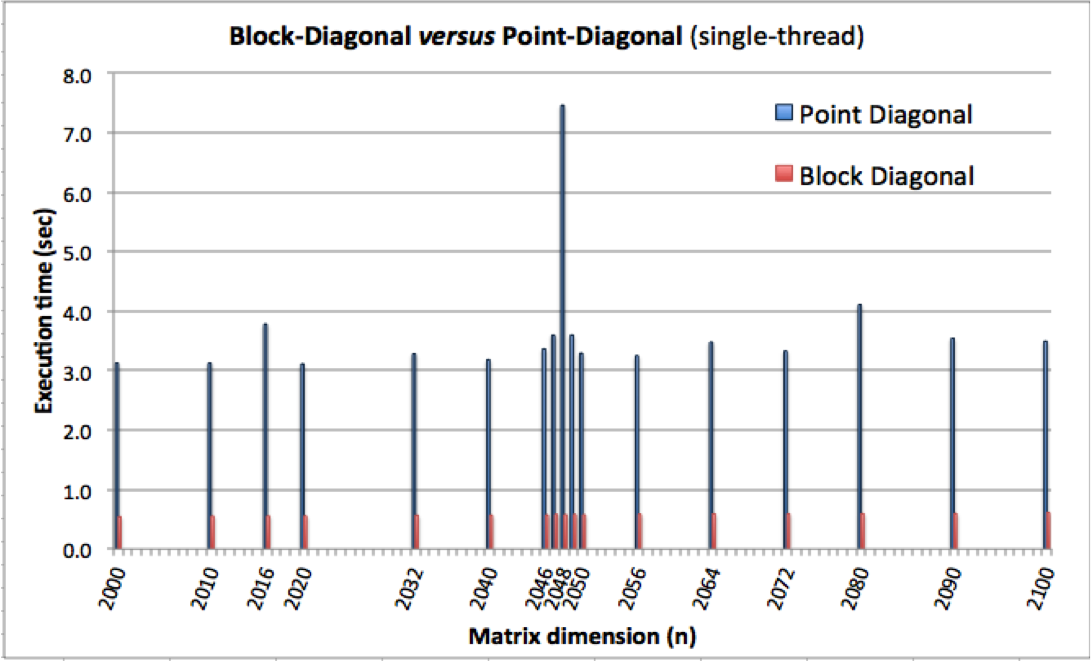
\includegraphics[width=0.9\textwidth]{assets/images/multicore/matrix-variations.png}
		\end{center}
		\caption{Execution time sensitivity for both point and block methods, using diagonal strategy}
		\label{fig:multicore:sensitivity}
	\end{figure}

	\Cref{fig:multicore:block:diagonal:speedup:accumulated} shows the speedup achieved only from blocking when using the diagonal strategy. This speedup is better noticed when using only one thread, since both strategies scale well. The accumulated speedup from both blocking and multithreading shows highly significant speedups, which are even greater when using special specific matrix sizes (\cref{fig:multicore:block:diagonal:speedup:accumulated:strange}).

	\begin{figure}[hp]
		\begin{center}
			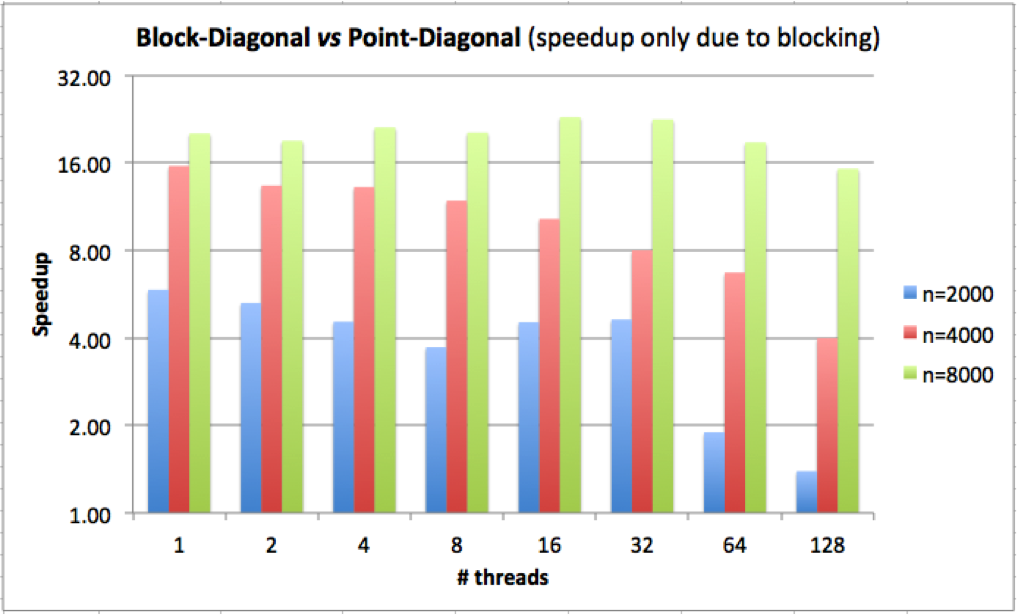
\includegraphics[width=0.9\textwidth]{assets/images/multicore/diagonal-speedup.png}
		\end{center}
		\caption{Speedups achieved with blocking for diagonal strategy}
		\label{fig:multicore:block:diagonal:speedup}
	\end{figure}

	\begin{figure}[hp]
		\begin{center}
			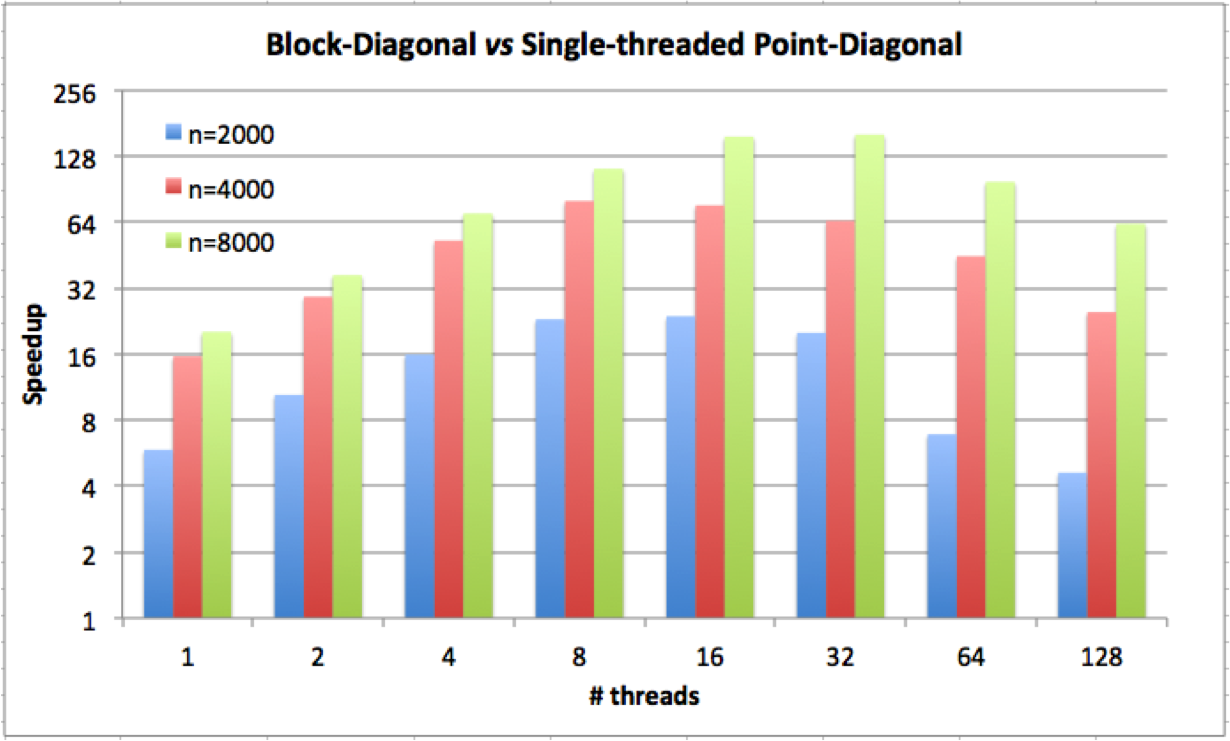
\includegraphics[width=0.9\textwidth]{assets/images/multicore/diagonal-block-stpoint-speedup.png}
		\end{center}
		\caption{Accumulated speedup achieved with blocking for diagonal strategy}
		\label{fig:multicore:block:diagonal:speedup:accumulated}
	\end{figure}

	\begin{figure}[hp]
		\begin{center}
			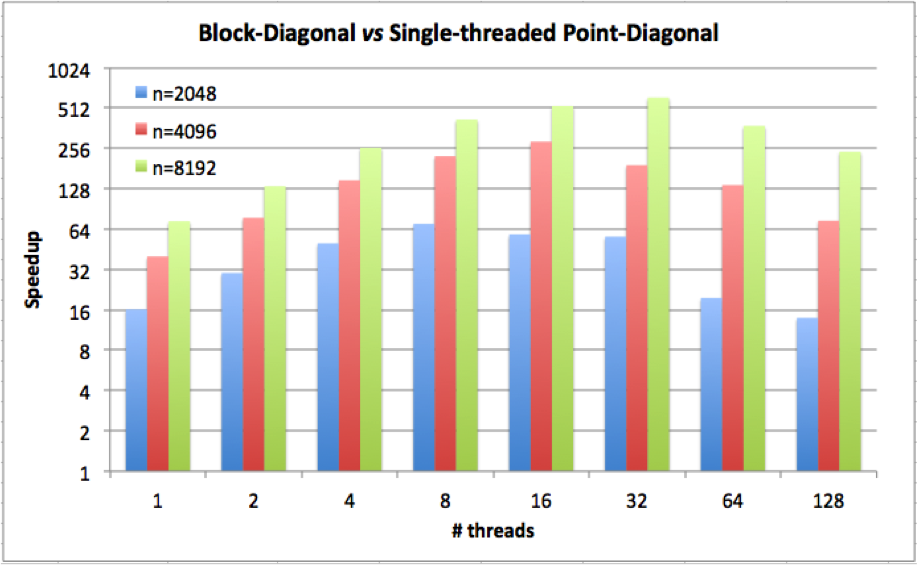
\includegraphics[width=0.9\textwidth]{assets/images/multicore/diagonal-block-stpoint-speedup-strange.png}
		\end{center}
		\caption{Accumulated speedups achieved with blocking for diagonal strategy (power of 2 sizes)}
		\label{fig:multicore:block:diagonal:speedup:accumulated:strange}
	\end{figure}
\end{document}
